
\documentclass{beamer}
\usepackage{graphicx}
\usepackage{caption}

\title{Intervention Simulation Results}
\author{Sol Kim}
\date{\today}

\begin{document}

\frame{\titlepage}

\begin{frame}
\frametitle{Overview}
\begin{itemize}
    \item Simulation for types A and B
    \item Interventions: Hand hygiene, Cleaning, Isolation
    \item Visualization of cumulative sum medians and IQR
\end{itemize}
\end{frame}

% Type A - hand
\begin{frame}{Type A - Hand Hygiene}
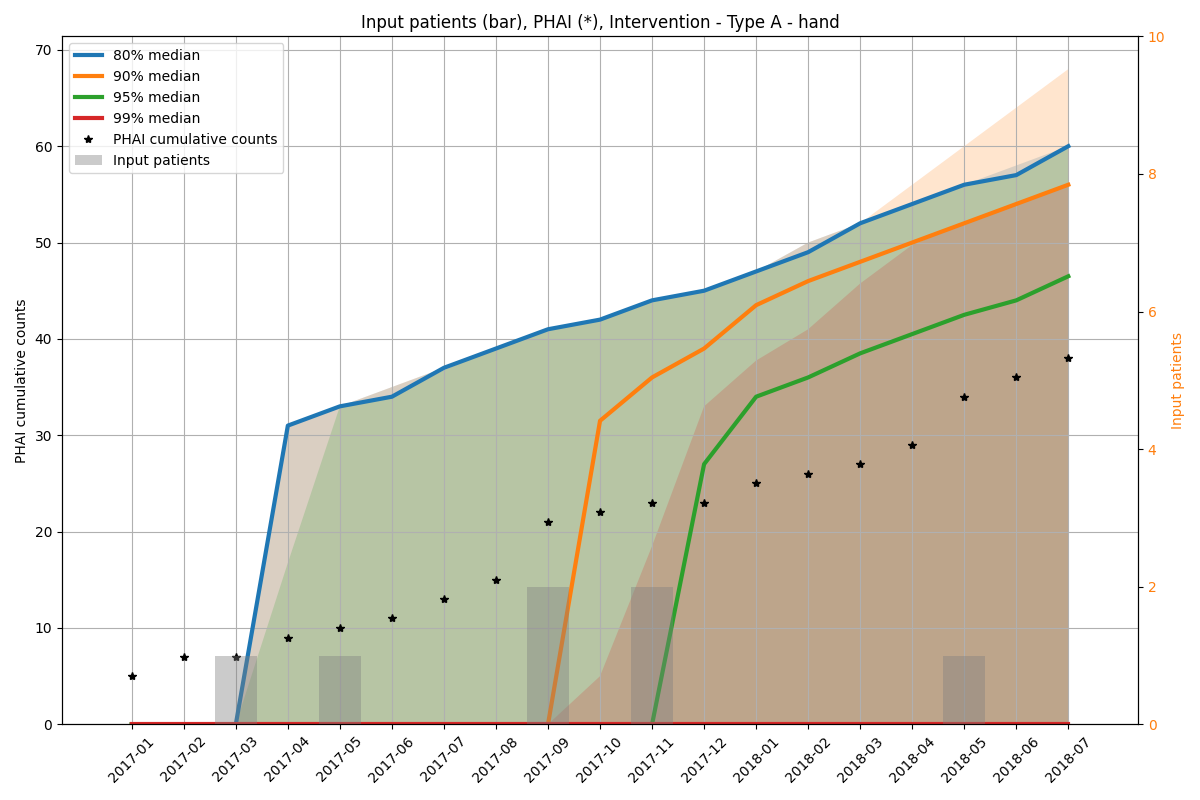
\includegraphics[width=0.9\linewidth]{../result/intervention/figureNtable/combined_A_hand.png}
\end{frame}

\begin{frame}{Type A - Hand Hygiene Boxplot}
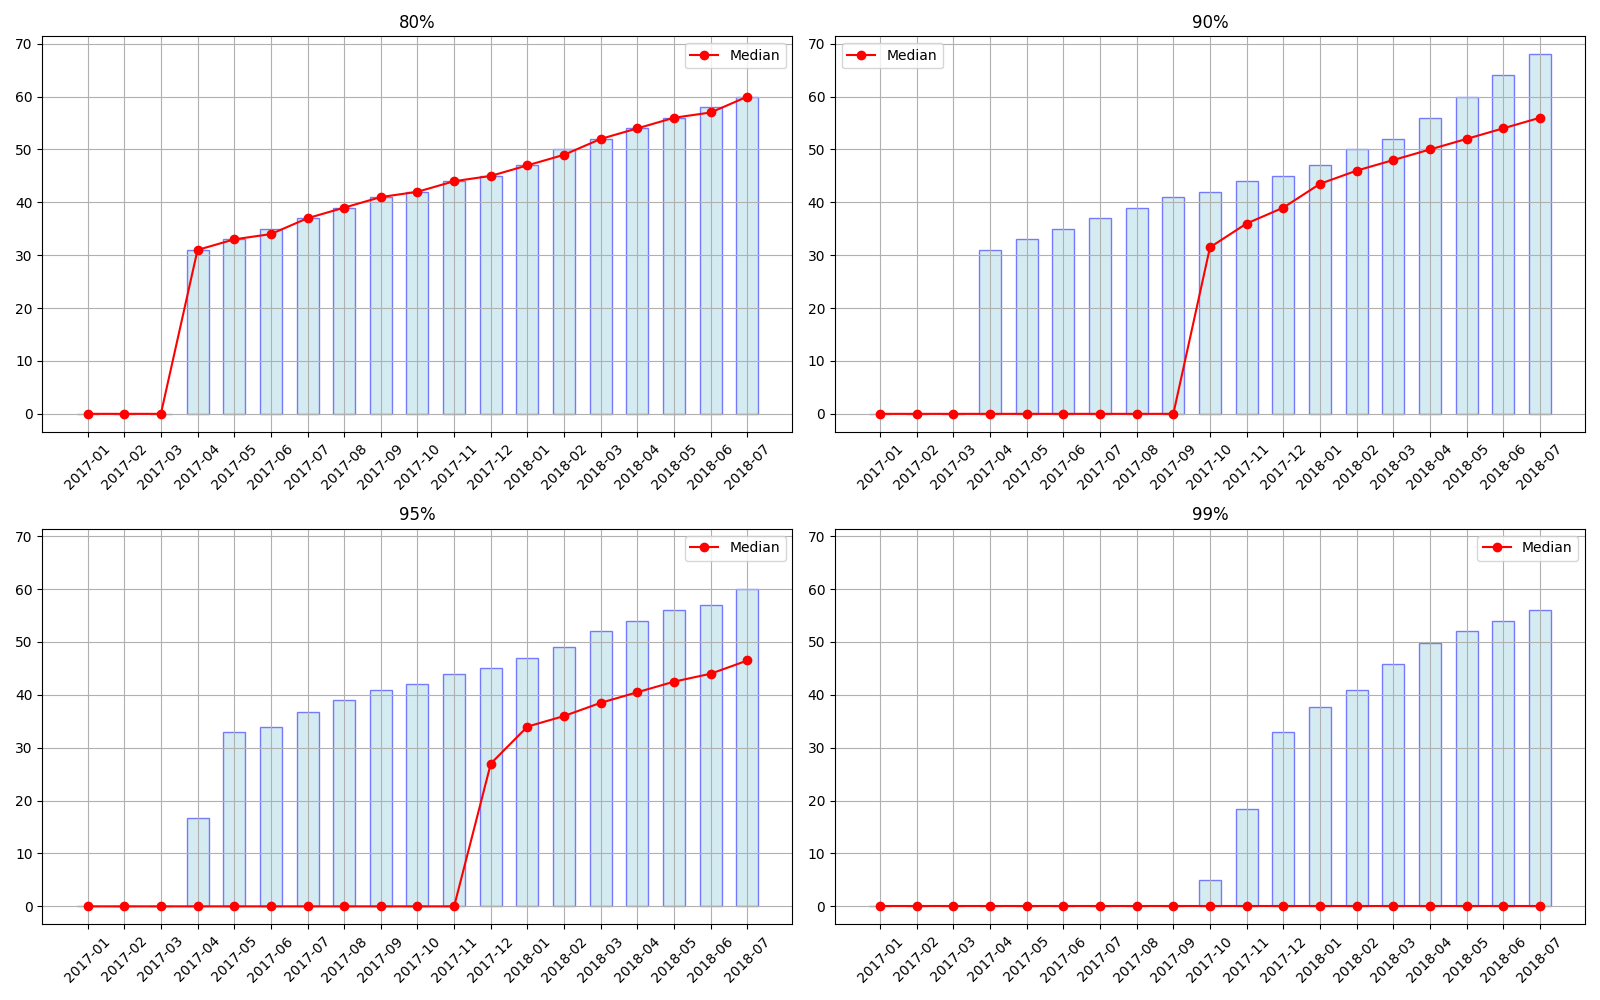
\includegraphics[width=0.9\linewidth]{../result/intervention/figureNtable/boxplot_A_hand.png}
\end{frame}

% Type A - clean
\begin{frame}{Type A - Cleaning}
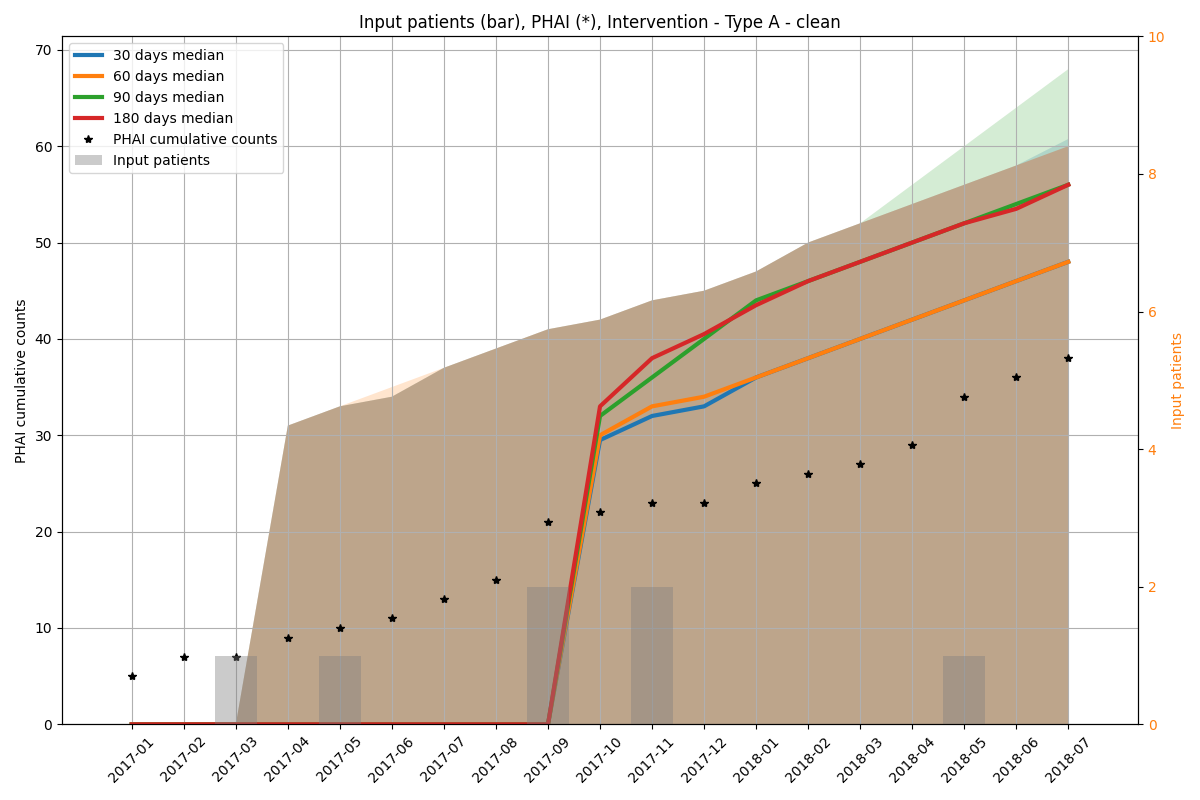
\includegraphics[width=0.9\linewidth]{../result/intervention/figureNtable/combined_A_clean.png}
\end{frame}

\begin{frame}{Type A - Cleaning Boxplot}
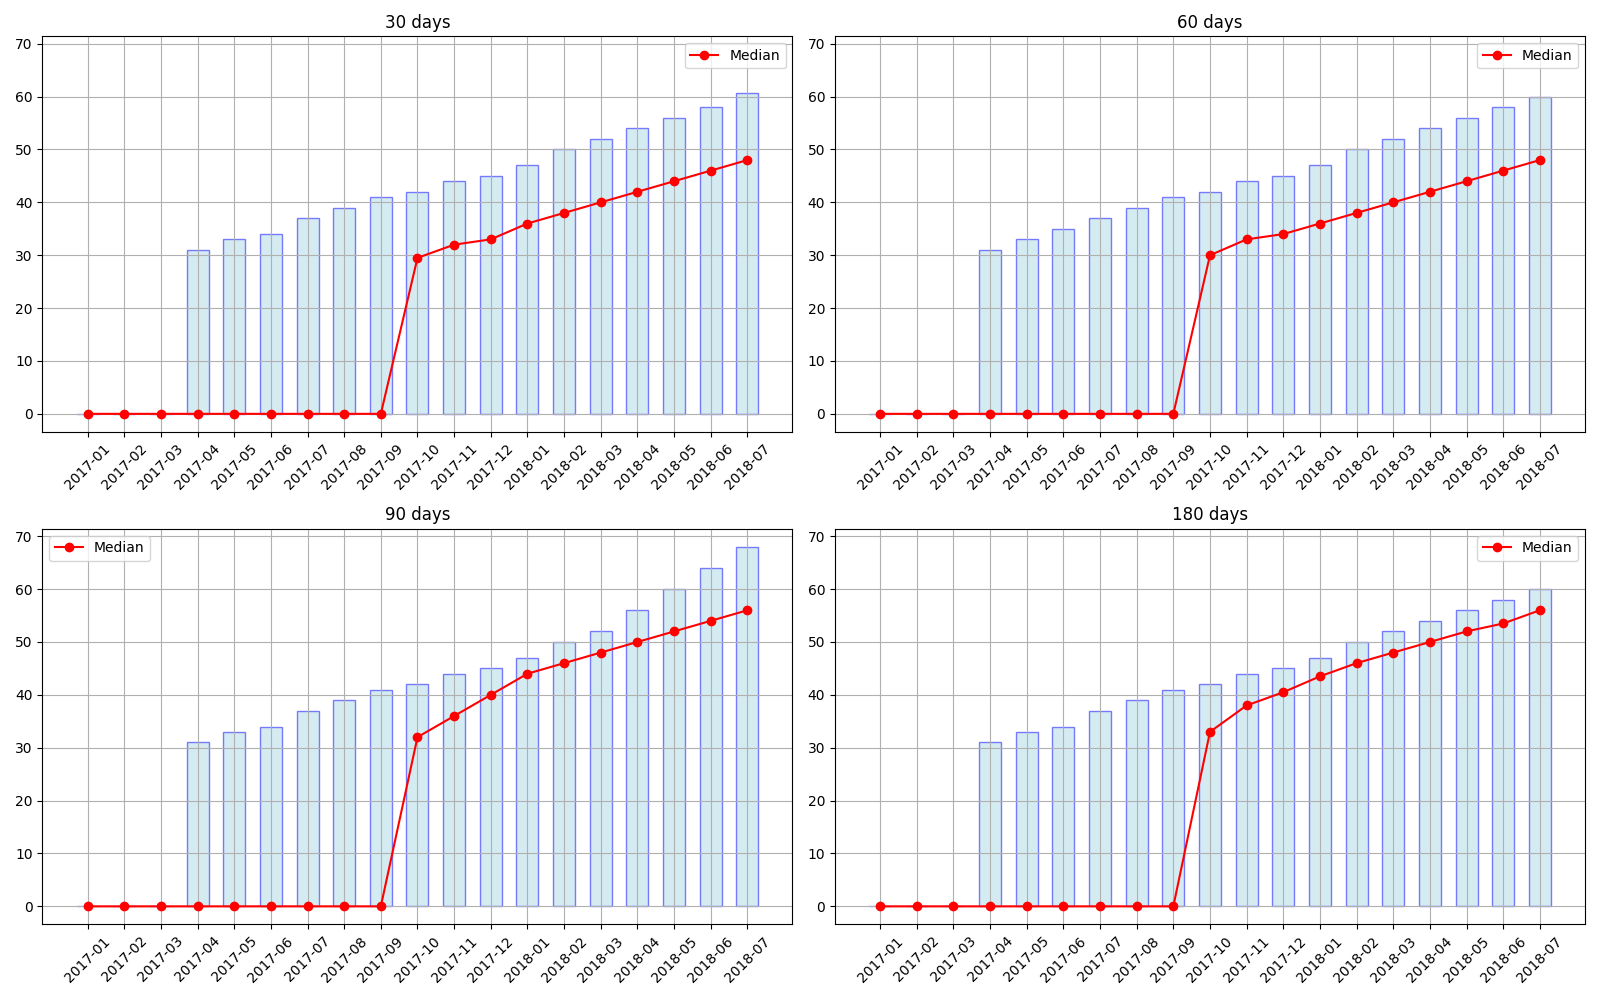
\includegraphics[width=0.9\linewidth]{../result/intervention/figureNtable/boxplot_A_clean.png}
\end{frame}

% Type A - iso
\begin{frame}{Type A - Isolation}
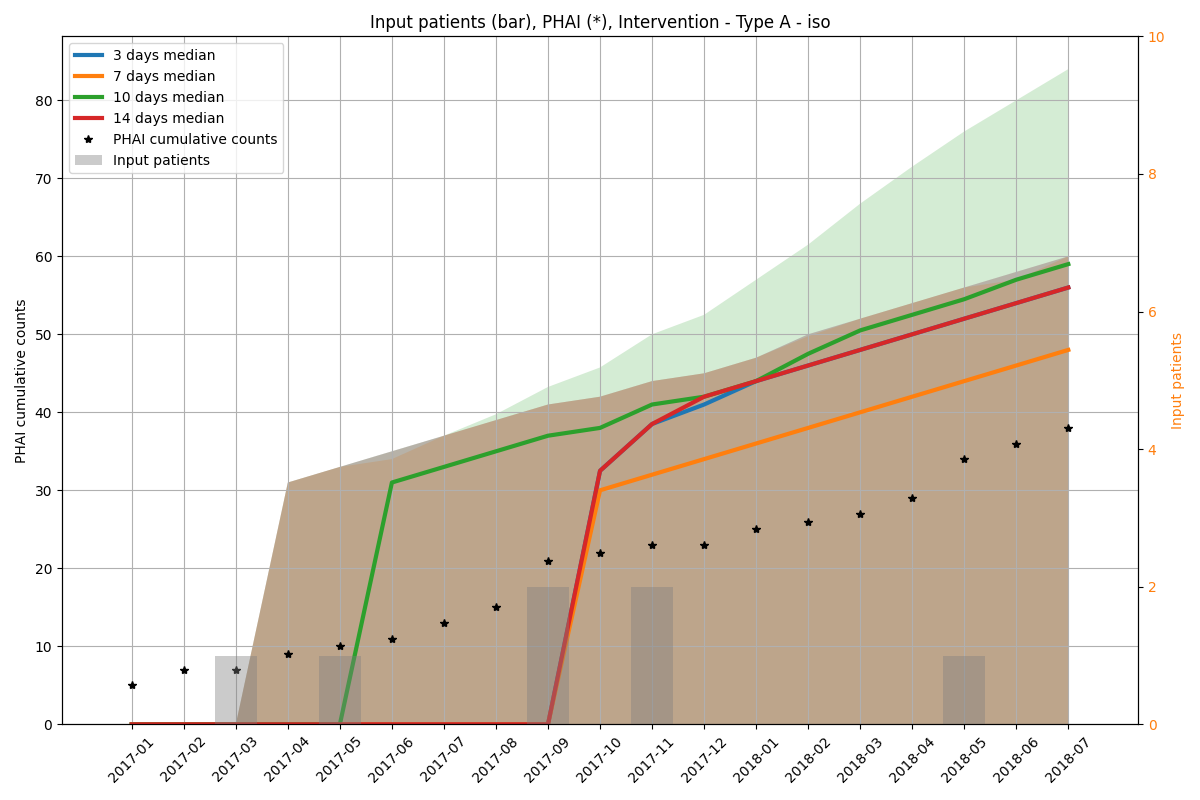
\includegraphics[width=0.9\linewidth]{../result/intervention/figureNtable/combined_A_iso.png}
\end{frame}

\begin{frame}{Type A - Isolation Boxplot}
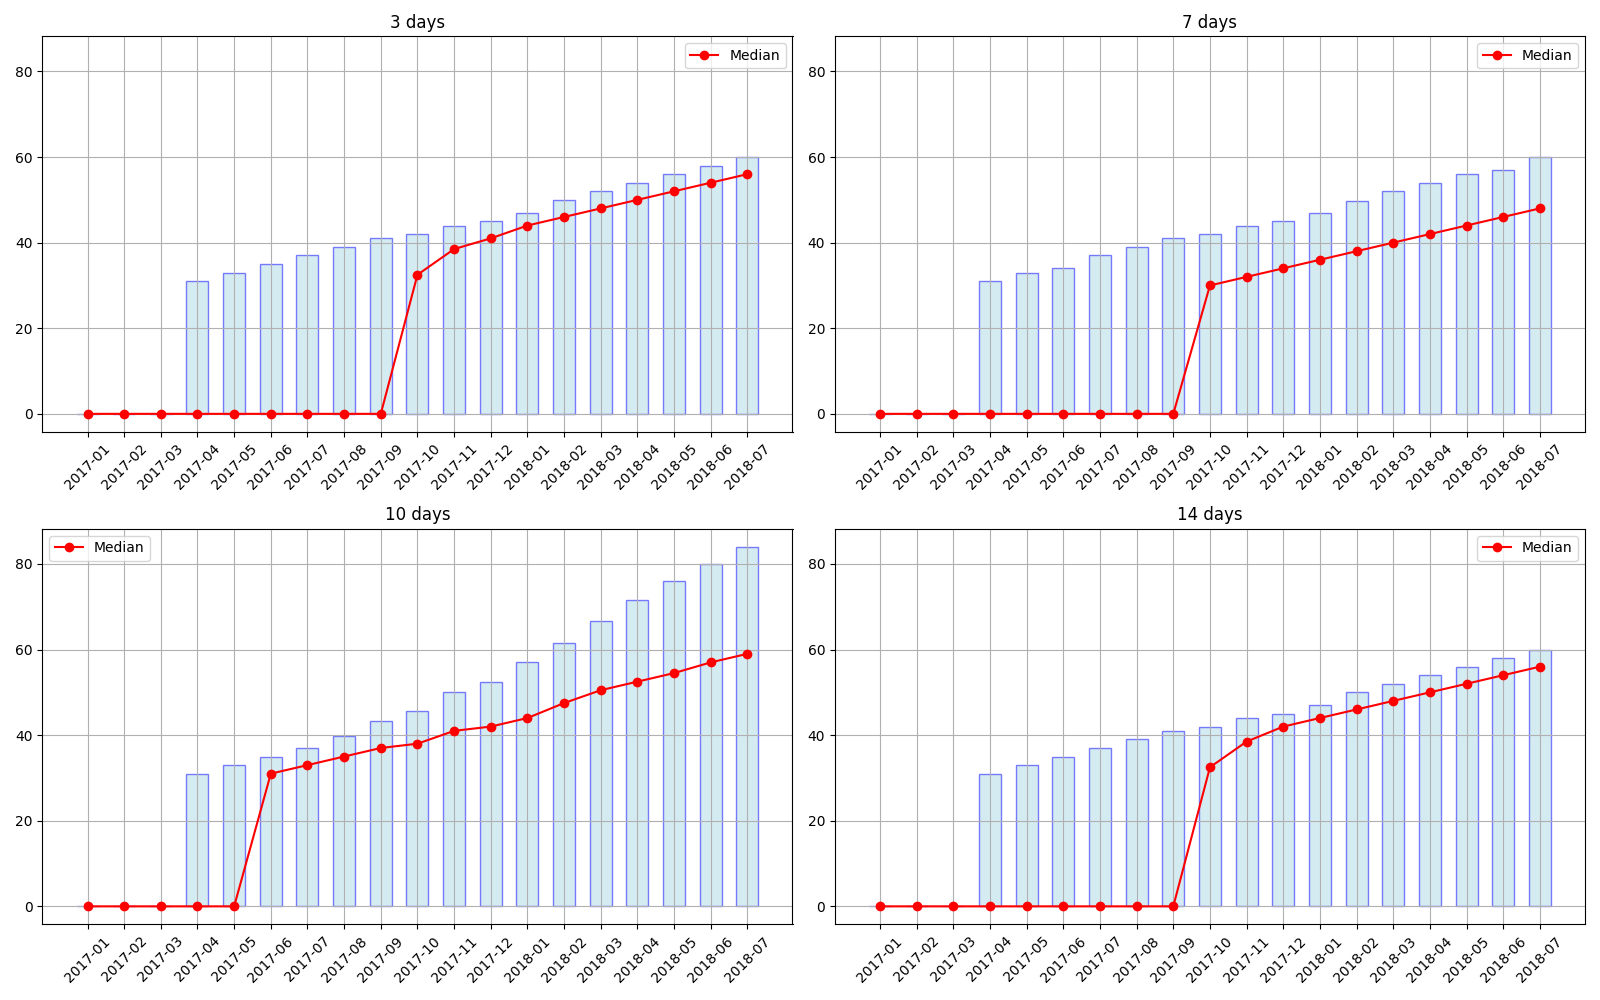
\includegraphics[width=0.9\linewidth]{../result/intervention/figureNtable/boxplot_A_iso.png}
\end{frame}

% Type B - hand
\begin{frame}{Type B - Hand Hygiene}
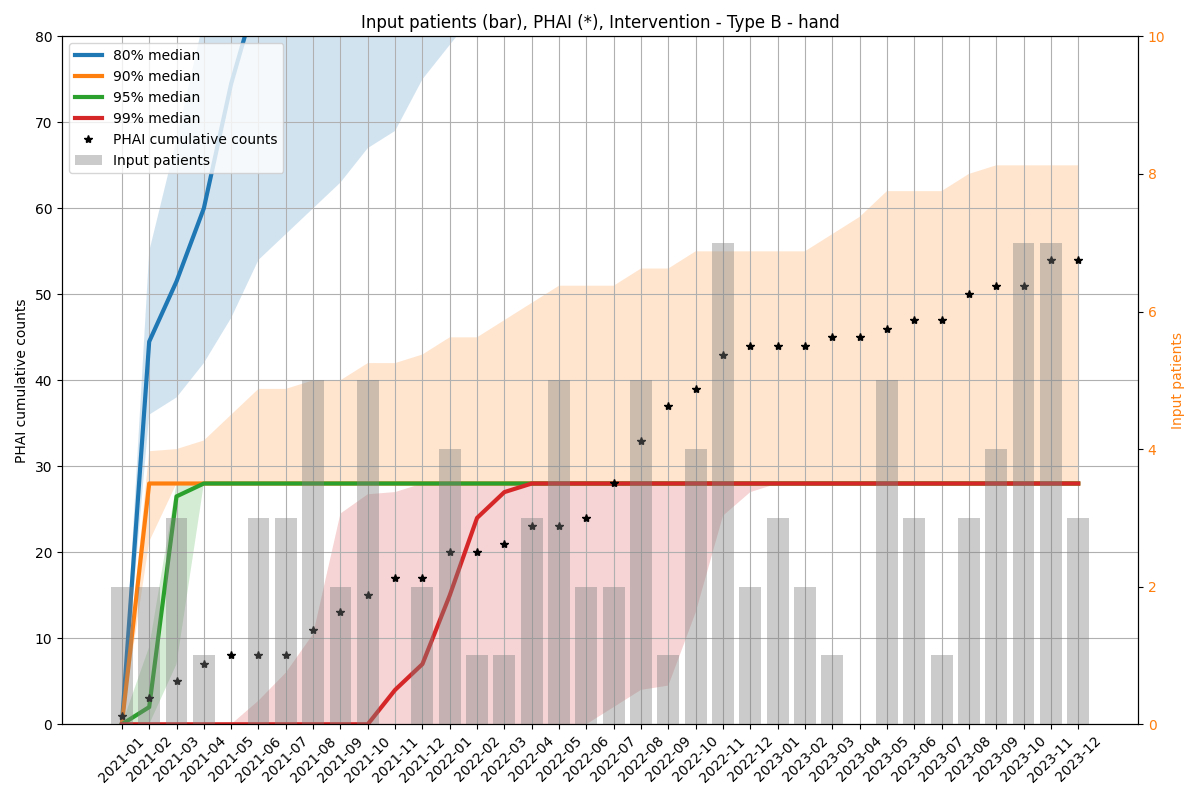
\includegraphics[width=0.9\linewidth]{../result/intervention/figureNtable/combined_B_hand.png}
\end{frame}

\begin{frame}{Type B - Hand Hygiene Boxplot}
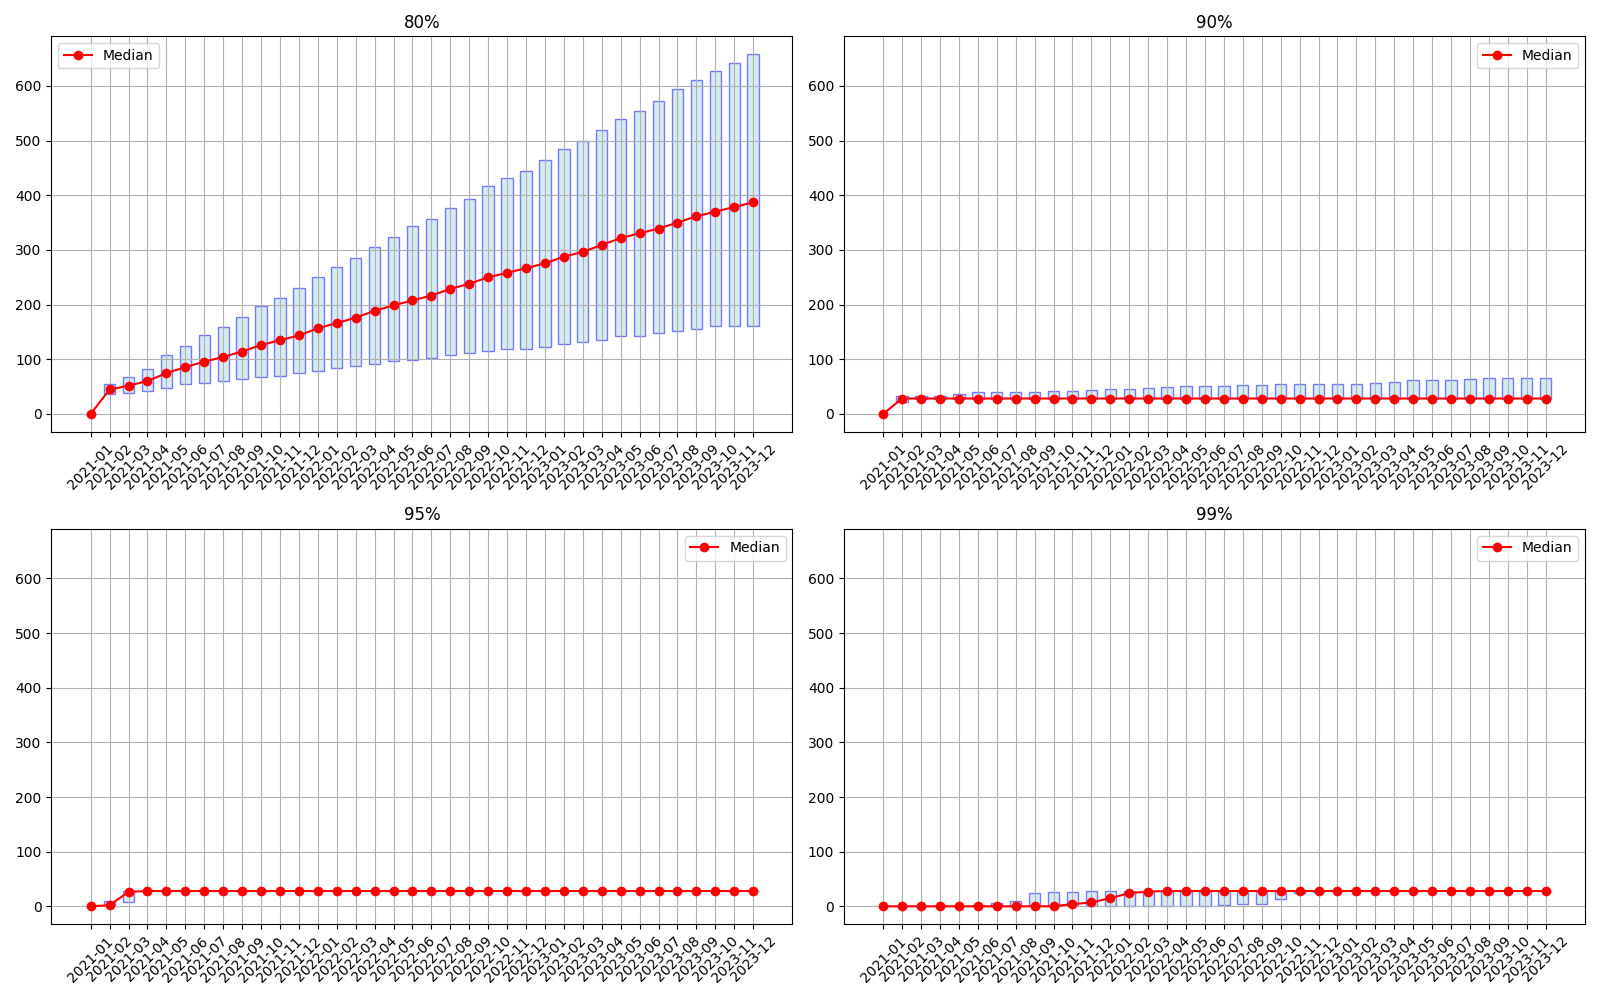
\includegraphics[width=0.9\linewidth]{../result/intervention/figureNtable/boxplot_B_hand.png}
\end{frame}

% Type B - clean
\begin{frame}{Type B - Cleaning}
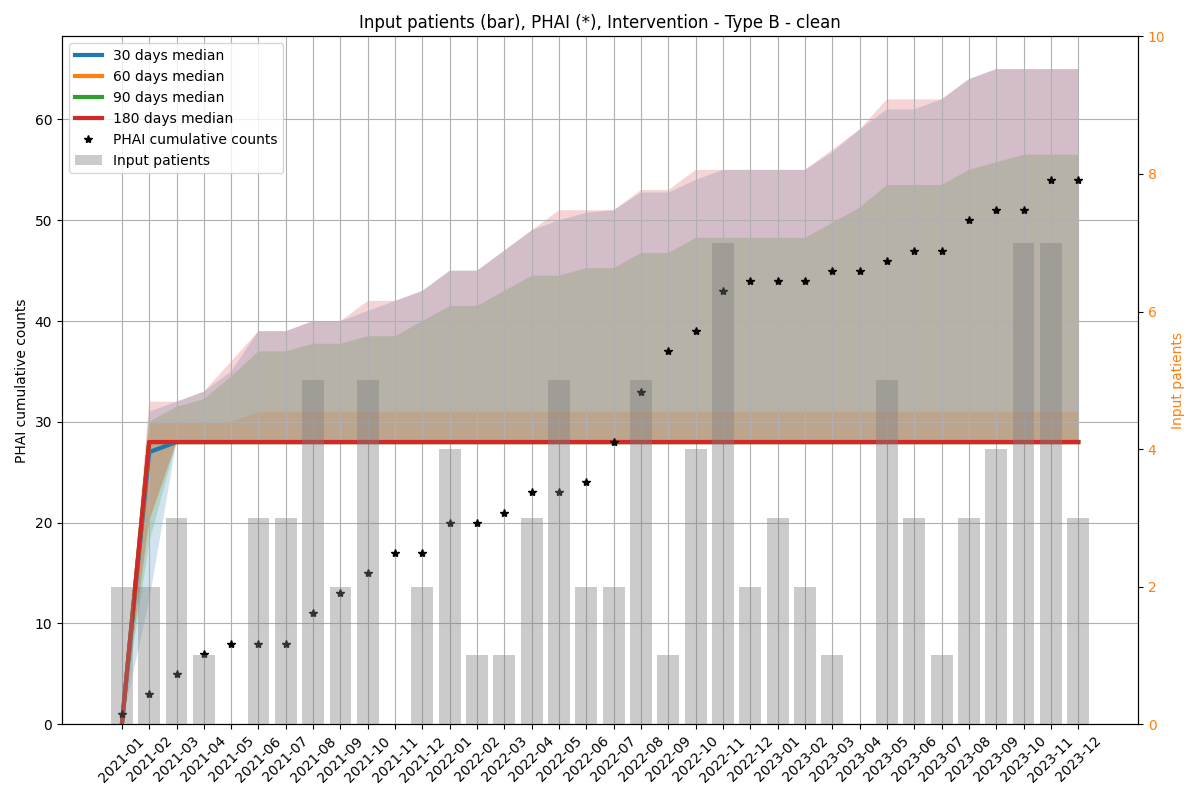
\includegraphics[width=0.9\linewidth]{../result/intervention/figureNtable/combined_B_clean.png}
\end{frame}

\begin{frame}{Type B - Cleaning Boxplot}
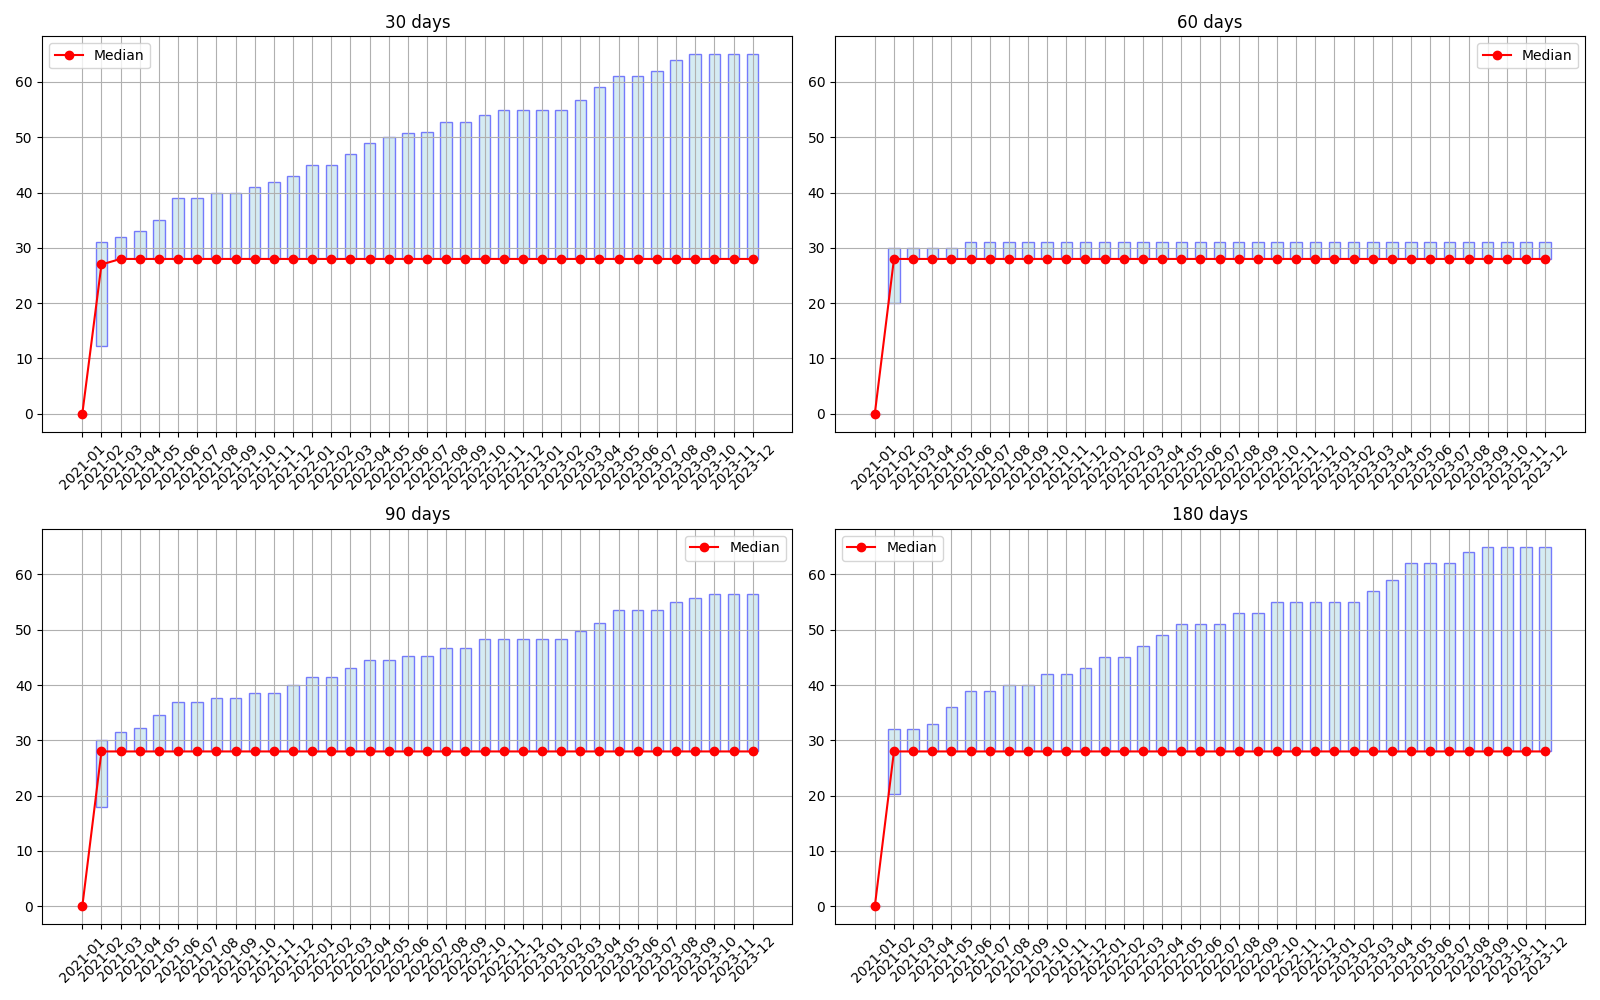
\includegraphics[width=0.9\linewidth]{../result/intervention/figureNtable/boxplot_B_clean.png}
\end{frame}

% Type B - iso
\begin{frame}{Type B - Isolation}
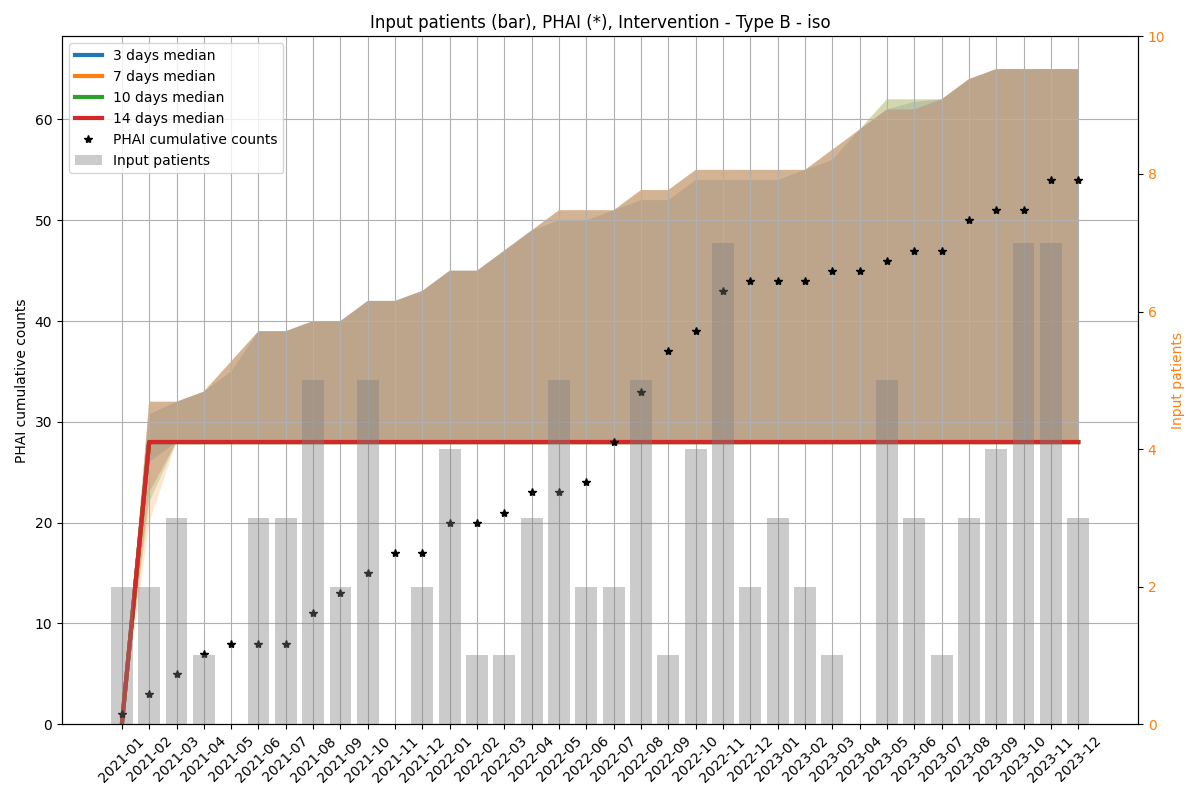
\includegraphics[width=0.9\linewidth]{../result/intervention/figureNtable/combined_B_iso.png}
\end{frame}

\begin{frame}{Type B - Isolation Boxplot}
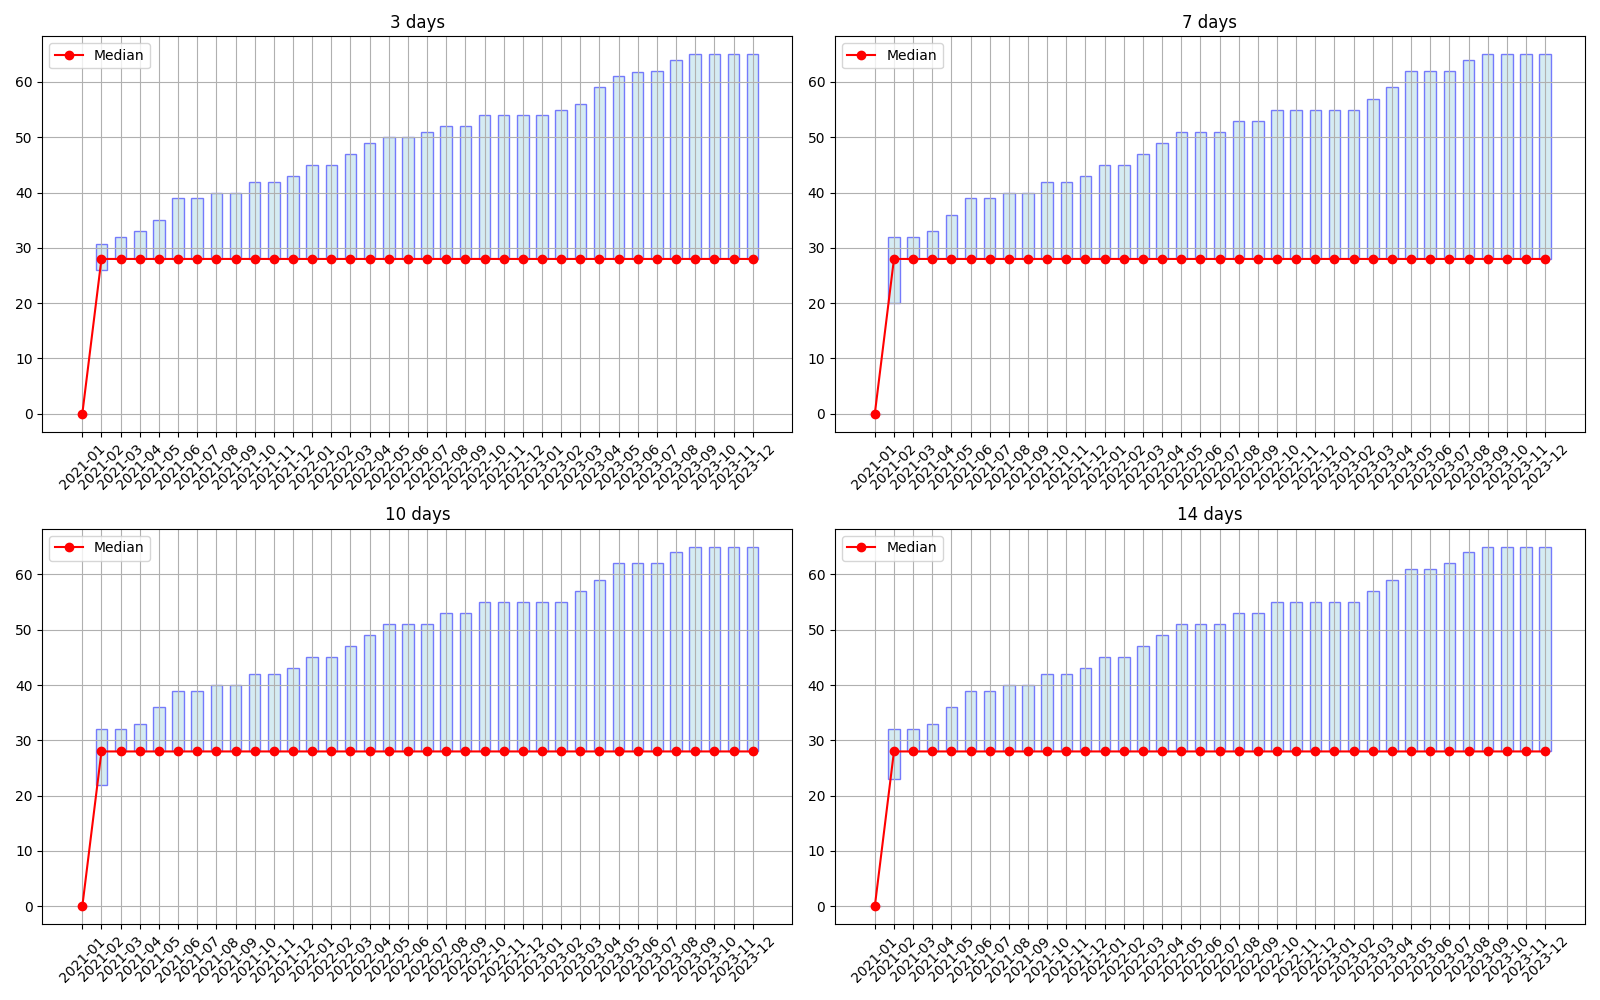
\includegraphics[width=0.9\linewidth]{../result/intervention/figureNtable/boxplot_B_iso.png}
\end{frame}

\begin{frame}
\frametitle{Summary}
\begin{itemize}
    \item Hand hygiene: strong early impact
    \item Cleaning: more sustained, gradual effect
    \item Isolation: rapid effect, important for outbreak containment
\end{itemize}
\end{frame}

\end{document}